\input{header}

\AtBeginSubsection[]
{
	\begin{frame}<beamer>
		\frametitle{Outline}
		\tableofcontents[current,currentsubsection]
	\end{frame}
}

\begin{document}
\begin{frame}[allowframebreaks,containsverbatim] \frametitle{Complexity of Nondeterministic TM}
  \begin{itemize}
\item Remember NTM is a decider if all branches halt on all inputs

\item Definition of NTM time complexity $t(n)$:

\item [] maximum \# of steps the machine uses for any path from root
  to a leaf

\item Theorem 7.11
\item [] Let $t(n) \geq n$. For a $t(n)$ NTM (single tape)

\item [] $\Rightarrow \exists \text{ a } 2^{O(t(n))}$ TM (single tape)
\item Assume $b$ is the maximal number of branches at each layer
\item Recall our way of doing the simulation is by the following
  three-tape TM

\begin{center}
  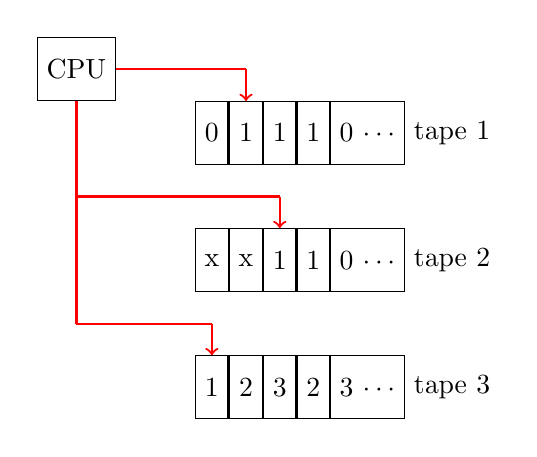
\begin{tikzpicture}[ampersand replacement=\&]
\matrix[nodes={minimum height=8mm}]     
{
  \node[draw](0) {CPU}; \& [1cm]  \& \node(1){} ; \&\&\& \& \\
  \& \node[draw]{0}; \& \node[draw](a){1}; \& \node[draw]{1}; \& \node[draw]{1};  \& \node[draw]{0 $\cdots$};  \& \node{tape 1};\\
\node(2){} ; \&  \&  \& \node(21){} ; \&\& \&\\  
\& \node[draw]{x}; \& \node[draw]{x}; \& \node[draw](b){1}; \& \node[draw]{1}; \& \node[draw]{0 $\cdots$}; \& \node{tape 2};  \\
\node(3){} ; \& \node(31){} ; \&  \&\& \& \&\\
\& \node[draw](c){1}; \& \node[draw]{2}; \& \node[draw]{3}; \& \node[draw]{2}; \& \node[draw]{3 $\cdots$}; \&  \node{tape 3}; \\
};

\draw [-,red,thick] (0) -- (1.center) ;
\draw [->,red,thick] (1.center) -- (a) ;
\draw [-,red,thick] (0) -- (2.center) ;
\draw [-,red,thick] (2.center) -- (21.center) ;
\draw [->,red,thick] (21.center) -- (b) ;
\draw [-,red,thick] (0) -- (3.center) ;
\draw [-,red,thick] (3.center) -- (31.center) ;
\draw [->,red,thick] (31.center) -- (c) ;
\end{tikzpicture}
\end{center}

\item We use a breadth-first way for the simulation
\item That is, after one layer is finished, we do the next

\item Tape 3: a path from root to a node

\item Total number of nodes in the tree:
\begin{equation*}
  O(b^{t(n)})
\end{equation*}

\item Tape 2: run the original input $w$ from root to one node in the
  tree

\item Cost of running from root to one node in tape 2: $O(t(n))$

\item Cost to update contents of tape 3: $O(t(n))$
\item []
  Recall that tape 3 has
  \begin{alltt}
1
2
3
11
...
333
111
...
\end{alltt}
\item Total time:
  \begin{equation*}
    \begin{split}
& \# \text{ nodes } \times \text{ cost per node}\\      
= &   O(b^{t(n)}) \times O(t(n)) = 2^{O(t(n))}
\end{split}
\end{equation*}
\item Note that in the above equality we used
  \begin{equation*}
    \begin{split}
&      b^{t(n)} \times t(n)
      =    2^{\log_2 (b^{t(n)} t(n))}
\\
= & 2^{(\log_2 b)t(n) + \log_2 t(n)} = 2^{O(t(n))}
    \end{split}
  \end{equation*}

\item This is by a 3-tape TM
\item To use a single-tape TM to simulate a 3-tape one, we need
  \begin{equation*}
(2^{O(t(n))})^2
= 2^{O(t(n))}
\end{equation*}
cost because
\begin{equation*}
  (2^{O(t(n))})^2
\leq (2^{ct(n)})^2
= 2^{2ct(n)} 
= 2^{O(t(n))}
\end{equation*}
\end{itemize}\end{frame}

\end{document}
